%!TEX root = ../tommaso-thesis.tex
%!TEX spellcheck = en_US


%-------------------------------------------------------------------------------------------
% Research Questions and Results
%
\newcounter{RQCounter}
\newcounter{RQACounter}

%Pass in label for rq, then rq
%

\newcommand{\RQ}[2]{%
\refstepcounter{RQCounter} \label{#1}
 \begin{framed}
  % \begin{examplebox}
   \textbf{RQ\arabic{RQCounter}.}~#2
  % \end{examplebox}
\end{framed}
}


% \chapter{What Makes a Satisficing Bug Report?}\label{ch:model}
\coolchapter{What Makes a Satisficing Bug Report?}{}{ch:model}


To ensure quality of software systems, developers use bug reports to track defects.
It is in the interest of users and developers that bug reports provide the necessary information to ease the fixing process.
Past research found that users do not provide the information that developers deem \emph{ideally useful} to fix a bug.
This raises an interesting question: What is the \emph{satisficing}\footnote{Satisficing is a neologism coined by Simon~\cite{Simo57,Simo01} combining the verbs {\em to satisfy} and {\em to suffice}, and it is used to describe a solution that is roughly satisfactory and meets some criteria of sufficiency and is better than an optimal solution that would be too complex or would imply too strong constraints.} information to speed up the bug fixing process?

We conducted an observational study on the relation between provided report information and its lifetime, considering more than 650,000 reports from open-source systems using popular bug trackers.
We distilled a meta-model for a \emph{minimal} bug report, establishing a basic layer of core features.
We found that few fields influence the resolution time and that customized fields have little impact on it.
We performed a survey to investigate what users deem easy to provide in a bug report.

\structure
In \secref{sec:model-intro} we discuss what we should expect from a bug report.
\secref{sec:model-method} presents our research method and introduces our research questions, that we answer in \secref{sec:model-approach}.
In \secref{sec:model-discussion} we discuss the meaning of our findings and how our work can be extended, while in \secref{sec:model-summary} we summarize and conclude the chapter.

\newpage


%%%%%%%%%%%%%%%%%%%%%%
\section{Good Bug Reports vs. Real Bug Reports}\label{sec:model-intro}
%%%%%%%%%%%%%%%%%%%%%%

When users file a bug report for a software project, their main hope is that developers will fix it quickly, to minimize its impact.
But what information should they provide to make this happen? There is a stark mismatch between what developers perceive as \emph{optimally} useful in this respect (\ie steps to reproduce, stack traces, and test cases) and what users are effectively able, or sometimes just willing to provide, when filing a bug report~\cite{Zimm2010a}.

Bug tracking systems and software projects should define a reasonable common ground for information to be provided in bug reports, so that it is not too demanding for users, yet provides enough information to developers.
Nevertheless, considering what popular issue trackers and projects (\eg \emph{Bugzilla}, \emph{JIRA}, \emph{FogBugz}, and the issue tracker provided with \emph{GitHub}) demand from users, we see that it is quite diverse and specialized.
In particular, each bug tracking system provides a core set of common fields, which are often complemented with additional fields.
Such  fields may reflect requirements for specific domains, or represent additional data customizable by project owners.

For example, the commercial issue tracker JIRA defines several fields that describe in detail aspects pertaining to the time management of issues, while the GitHub issue tracker provides a minimal (and sometimes criticized\footnote{\url{https://github.com/dear-github/dear-github}}) model that, together with the integration with the Git versioning system, conceives a bug report as a conversation among developers, fostering the philosophy of collaborative development proposed by GitHub~\cite{Thun2013}.

Overall, there is currently no consensus among software projects and creators of bug reporting systems on essential mandatory fields to be filled by users in each report, optional fields that give useful additional information, and free space for users willing to provide more detailed descriptions.

Our vision is to define the minimum set of information needed to describe a software defect, to clarify what should be required by each bug reporting system.
In this chapter, we make a step in this direction: We investigate what makes a \emph{satisficing} bug report.
We move from defining a good or more precisely an \emph{optimal} bug report and adopt a more pragmatic view on what users should provide.

%This goal requires to consider the amount of required information, the reliability of the data, and the evolution of the report during its lifetime.

We conduct our investigation in three steps: \begin{inparaenum}[(1)]
\item We investigate what users and developers perceive as \emph{difficult} in writing a report, by means of an online questionnaire;
\item we investigate the usage and evolution of issue tracker data, by means of a large-scale quantitative analysis of the status changes in submitted bug reports and the impact that customized fields have on the resolution of a defect;
\item we study which fields developers use to describe defects, by means of a further quantitative analysis on the lifetime of reports in relation to the evolution of report's state and its \emph{completeness} in its core and customized fields.
\end{inparaenum}

Our results show that providing more fields in a report relates to the fixing time: In particular, the bug reports with longer descriptions tend to be solved quicker.
While this might be intuitive, issue trackers still do not emphasize this aspect during the submission of a new bug report, putting the accent on the customization capabilities of the platform.
At the same time, the project-specific bug report fields have little impact to the fixing time.
This chapter provides insights on the current issue tracking practices and defines guidelines in building the foundations for a new model of an issue tracking system.

\newpage
The contributions presented in this chapter are:

\begin{itemize}[$\circ$]

\item A survey that identifies the components of a bug report considered difficult to provide by users (\secref{sec:model-survey}).

\item A dataset of 650,000 bug reports, collected from the issue trackers of \bzilla and \jira (\secref{sec:model-collection}).

\item The model for a minimal bug report, that puts the emphasis on the shared components of a bug report (\secref{sec:model-model})

\item An analysis of the usage of the fields in an issue tracker, from active open source projects (\secref{sec:model-fields}).

\end{itemize}




% %%%%%%%%%%%%%%%%%%%%%%%%%%%%%%%%%%%
% \section{Issue Tracking Systems}\label{sec:model-bugtrackers}
% %%%%%%%%%%%%%%%%%%%%%%%%%%%%%%%%%%%
%
% To obtain an overview of the salient features of issue trackers, we briefly present four platforms, selected by importance and overall adoption in open-source systems: \bzilla, \jira, the \gth issue tracker and \fbz.
%
% \subsubsection{Bugzilla} One of the oldest and most popular issue tracking systems that influenced many other issue trackers.
% Developed by the Mozilla Foundation, it is used both by open source projects\seeurl{https://www.bugzilla.org/installation-list/} (\eg Linux) and by industrial and government customers (\eg NASA).
% The Mozilla Foundation itself uses \bzilla to manage the issues of its projects, like Firefox.
% \bzilla includes several fields, allowing for a great level of detail in specifying an issue.
% However, such a freedom of choice also produces a complex interface where many of the values are often left empty, or set to their default value.
% \figref{fig:bugzilla-interface} shows a typical submission form with both fields for fixed-option choices and text boxes for narrative (\eg to describe how to reproduce the bug).
%
% \begin{figure}[ht]
% \centering
%   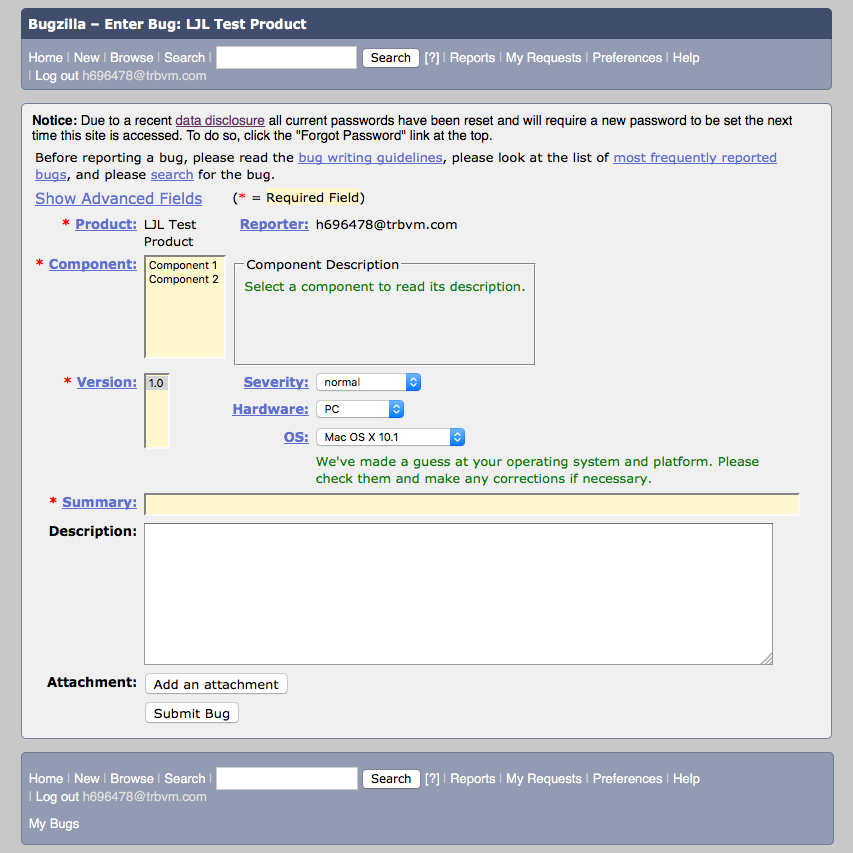
\includegraphics[width=.9\linewidth]{model/bugzilla}
%   \caption{Bugzilla Submission Form}
%   \label{fig:bugzilla-interface}
% \end{figure}
%
% \subsubsection{JIRA} A successful commercial bug reporting systems used by several customers like Twitter, Linkedin, and Ebay.\seeurl{https://www.atlassian.com/company/customers} \jira supports the same model as \bzilla, augmenting its capabilities with a polished user interface and a tight integration with other development tools, especially with the version control system.
%
%
% \subsubsection{GitHub} A popular web-based \textsc{Git} repository hosting service, used for the development of several popular open source projects.
% Together with the \textsc{Git} hosting service, \gth offers a simple issue tracker to manage the defects during development.
% \figref{fig:github-interface} shows the interface of the \gth bug submission form.
%
% \begin{figure}[ht]
% \centering
%   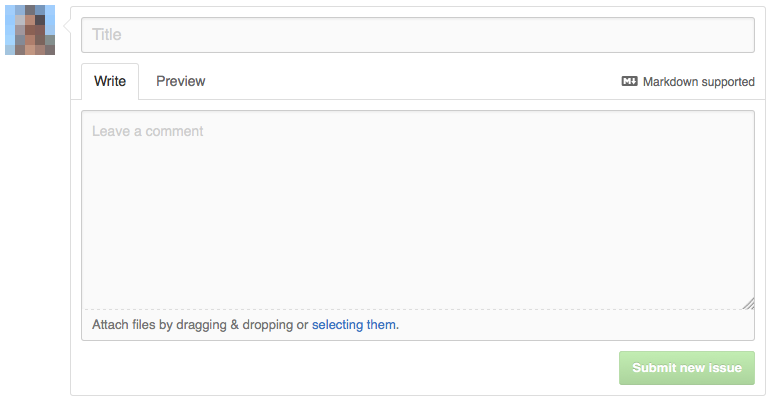
\includegraphics[width=\linewidth]{model/github}
%   \caption{GitHub Bug Submission Form}
%   \label{fig:github-interface}
% \end{figure}%
%
% \gth adopts a simplified model of a bug report and a strong integration with the source code (thus giving the possibility to link issues with specific commits).
%
% \subsubsection{FogBugz} In this system, the model of a bug report is similar to \bzilla, but more polished and user-friendly, due to its clean user interface and filtering capabilities.
% Differently from \gth, \fbz\seeurl{https://www.fogcreek.com/fogbugz/} does not simplify the report model, but it lets users add custom filters and views.

\subsubsection{Reflection} To understand the essential traits of bug reports, we analyze how the data included in bug reports influences their lifetime.
We next analyze the features of a set of bug reporting systems, to distill a model of common/specific fields for their bug reports.
This model serves as a basis for further empirical analysis, to determine how these commonalities and customizations influence the life of the reports.


%%%%%%%%%%%%%%%%%%%%%%%%%
\section{Research Method}\label{sec:model-method}
%%%%%%%%%%%%%%%%%%%%%%%%%

To determine what makes a satisficing bug report, we first need a way to rate the quality of a bug report, then we can conduct quantitative analysis to determine which features relate with higher quality.
Measuring the quality of bug reports is hard to do in an automated and unbiased way.
For this reason, researchers proposed different metrics to measure it~\cite{Hooi2007}, all with their limitations, but reasonable enough to be realistic.
In this work, we decide to consider the \emph{lifetime} of a bug report (\ie the time between the opening and resolution of a defect) as a viable proxy for its quality rating, as the time spent dealing fixing software defects is crucial in reducing the time the system contains a problem.
Limitations of this proxy metric include the fact that the trivial bugs, or the non-issues, are the ones that require less time to fix, and that the severity can also have a not negligible impact on how quickly developers decide to fix a problem.
Nevertheless, the information shared in the bug report has to be satisficing enough to let developers understand whether it is a trivial fix, an urgent matter, or something that can wait longer.
For this reason, we find lifetime of a bug report a useful approximation in aggregate statistical analyses to provide a high-level view over bug repositories.

We investigate how users and developers use issue tracking systems and the impact that the provided information has on the lifetime of a bug report.
According to Zimmermann \etal the information provided by submitter can be partial or incorrect~\cite{Zimm2010a}.
To understand what is reasonable for a user to provide in a report, we conducted a survey asking developers what they think are the difficult elements to provide.
We then focus on two of the main components that compose a bug report: (1) its state and (2) the core and optional attributes, to understand how the provided data is used.

%%%%%%%%%%%%%%%%%%%%%%%%%%%%%%%
\subsection{Research Questions}\label{sec:model-questions}

When collecting information about software defects, it is important to know when the submitted data is reliable and accurate.
Our goal is to investigate what  users can easily provide and what is harder to obtain; we structure our investigation into the following question:

\RQ{rq1}{What are the elements that are perceived as difficult to provide when reporting a defect?}

To understand the relationship between what is described in a bug report and its lifetime, we have to consider the different kind of data that reports can provide.
This is not trivial, because different platforms offer different fields to provide information, with different meaning and values.
As a first step for our quantitative evaluation, we investigate how to define a meta-model to comprehensively describe information stored across different issue reporting systems:

\RQ{rq2}{What is a comprehensive unified meta-model for describing data from different bug tracking systems?}

After having defined the meta-model, we can quantitatively investigate several aspects of reports related to their lifetime and evolution.
During development, a bug report changes its state, sometimes several times, ideally converging to a closed state.
The changes in the state of a report are important to understand its evolution~\cite{DAmb2007b}.
We are interested in considering the evolution of the states and see whether the aggregate of these changes can provide knowledge on the inner logic of an issue tracker.
This leads to the following question:

\RQ{rq3}{What are the most frequent states and state transitions in bug reports?}

Together with a state, a bug report comes with a set of attributes that describe the properties of a report.
These attributes can also be defined by the users, to create project-specific customized fields.
We investigate the completeness of core and custom fields with respect to the lifetime of a bug, considering the following research question:

\RQ{rq4}{Does the completeness of standard and project-specific attributes in a bug report relate to its lifetime?}

To answer our questions, we both run a survey (\secref{sec:model-survey}) and we collect, model, and analyze a large dataset of bug reports from open source projects (\secref{sec:model-collection}).

%%%%%%%%%%%%%%%%%%%%%%%%%%%%%%%%%%%%
\subsection{Online Questionnaire} \label{sec:model-survey}

Zimmerman \etal asked users and developers what they think are the useful elements in a bug report and how hard it is, in their opinion, to provide those elements~\cite{Zimm2010a}.
We proposed a similar questionnaire to the \emph{Pharo} open source community to further understand what it is reasonable to expect from users submitting a bug report.
The questionnaire is composed of two parts: \begin{inparaenum}[(1)]
\item We collect demographic information inquiring about expertise with programming and with submitting, handling, and fixing bug reports; and
\item we collect information about respondents' perception of how difficult it is to provide different kinds of information when submitting a bug report.
\end{inparaenum}
All the questions are formulated as statements (\eg ``It is easy to provide a description of the failure'') and the respondents have to declare their agreement using a 5-level Likert-type scale.
We map the results into an integer scale from $-2$ (\ie ``strongly disagree'') to $2$ (\ie ``strongly agree'').

\begin{table}[t]\small
\centering
\caption{Expertise of the participants of the survey (average)}\label{tab:survey}
\rowcolors{1}{tablefirstrow}{tablesecondrow}
\begin{tabular}{lr}
\rowcolor{tableheader} \textbf{Activity} & \textbf{Average} \\
\hline
Experience with Object Oriented programming languages & $1.5$ \\
Knowledge of Pharo & $1.3$ \\ \hline
Have often bug reports assigned & $-0.4$ \\
Often handle bug reports & $0.6$ \\
Often participate in discussion in bug reports & $0.3$ \\
Often submit bug reports & $0.7$ \\
\hline
\end{tabular}
\label{tab:survey-expertise}
\end{table}

We advertised the survey through the development mailing list of Pharo and we received a total of 22 complete responses.
\tabref{tab:survey-expertise} summarizes the respondents' expertise.
The respondents are experienced with object-oriented programming and with the Pharo IDE.
While they have experience in submitting and handling bug reports, their experience is lower in participating in discussions about bug reports and much lower in having reports assigned to them.
For this reason, we deem the respondents' sample to be in line with the aim of our survey.
In fact, we are especially interested in knowing the point of view of submitters of bug reports, rather than the view of the developers that ``consume'' these reports.


%%%%%%%%%%%%%%%%%%%%%%%%%%%%

\begin{table}[t]\small
\centering
\caption{Overview of the projects in the dataset}\label{tab:dataset-projects}
% \rowcolors{1}{tablefirstrow}{tablesecondrow}
\begin{tabular}{l|l|rrrrr}
 \rowcolor{tableheader}
 &               & \multicolumn{5}{c}{{\bfseries Issues}} \\
%Ecosystem
 \rowcolor{tableheader}
 & Project & First & Last & Count & Age (days) & Frequency \\
\hline
\multirow{9}{*}{\rotatebox[origin=c]{90}{Apache}}
 & Cassandra & Mar 7, 2009 & Jul 8, 2015 & 9,723 & 2,314 & 5h 42m \\
 & Hadoop & Jul 24, 2005 & Jul 8, 2015 & 10,191 & 3,635 & 8h 33m \\
 & Lucene & Oct 9, 2001 & Jul 8, 2015 & 6,641 & 5,019 & 18h 8m \\
 & Maven & Nov 20, 2002 & Jul 23, 2015 & 4,663 & 4,628 & 23h 49m \\
 & Mahout & Jan 30, 2008 & Jun 25, 2015 & 1,752 & 2,702 & 37h 6m \\
 & Pig & Nov 2, 2007 & Jul 7, 2015 & 767 & 2,804 & 87h 44m \\
 & Sorl & Jan 25, 2006 & Jul 8, 2015 & 7,728 & 3,451 & 10h 43m \\
 & Zookeeper & Jun 6, 2008 & Jul 3, 2015 & 2,207 & 2,582 & 28h 4m \\
\hline
\multirow{6}{*}{\rotatebox[origin=c]{90}{Mozilla}}
 & Air Mozilla & Apr 14, 2009 & Jun 16, 2015 & 509 & 2,254 & 106h 16m \\
 & Bugzilla & Apr 15, 1998 & Jul 27, 2015 & 19,395 & 6,312 & 7h48m \\
 & Core & Mar 28, 1997 & Jul 17, 2015 & 292,358 & 6,684 & 33m \\
 & Firefox & Jul 30, 1999 & Jul 8, 2015 & 155,078 & 5,821 & 54m \\
 & Firefox for Android & Sep 11, 2008 & Jul 28, 2015 & 18,906 & 2,510 & 19m \\
 & SeaMonkey & Nov 10, 1995 & Jul 27, 2015 & 92,757 & 7,198 & 1h 51m \\
 & Thunderbird & Jan 2, 2000 & Jul 8, 2015 & 42,247 & 5,666 & 3h13m\\\hline
\end{tabular}
\end{table}

\subsection{Data Collection} \label{sec:model-collection}

To understand what users and developers collect and provide in bug reports, we mined the contents of the issue trackers of several software projects.
To collect real development data for our study, we consider the Apache Foundation and the Mozilla Foundation: Both platforms contain a considerable number of popular and active open source projects, with years of development history.
Moreover, both platforms host several projects tracked on public, dedicated bug trackers: Mozilla uses \bzilla, Apache uses \jira.
They offer a public \textsc{REST} API to access their repositories in \textsc{JSON} format, allowing for a clean and reliable data collection.

We built a downloader and an importer to collect the data, serialize the contents of each report, and store the polished data in a \textsc{PostgreSQL} database.
\tabref{tab:dataset-projects} describes our dataset.

The dataset contains more than 650,000 bug reports, $15\%$ of which were still open during the data collection phase.
\tabref{tab:dataset} shows an aggregated summary of the dataset we collected.
Each bug tracker has a different set of bug report states.

\begin{table}[h]\small
\centering
\caption{Contents of the dataset}
\rowcolors{1}{tablefirstrow}{tablesecondrow}
\begin{tabular}{l|rrr}
 \rowcolor{tableheader}
 & Apache & Mozilla & Total \\
\hline
%Projects & 8 & 7 & 15 \\
Open issues & 7,545 & 91,336 & 98,881 \\
Closed issues & 36,127 & 529,914 & 566,041 \\
Total Issues & 43,672 & 621,250 & {\bfseries 664,922} \\ \hline
\end{tabular}
\label{tab:dataset}
\end{table}

\tabref{tab:dataset-statuses} details them, for each tracker, with the counts of the bug reports for each state at the moment of the download.

\begin{table}[ht]\small
\centering
\caption{Different states of bug reports in \bzilla and \jira, with the count of the reports currently in each state and the total sum of all the times a bug report reached a state.}
\rowcolors{1}{tablefirstrow}{tablesecondrow}
\begin{tabular}{l|l|rr}
\rowcolor{tableheader}{\bfseries Tracker} & {\bfseries State} & {\bfseries Current} & {\bfseries Total} \\ \hline
JIRA & Closed & 21,847 & 22,460 \\
& Resolved & 14,280 & 33,386  \\
&  Open & 6,736 & 43,203 \\
&  Patch Available & 471 & 18,944 \\
&  Reopened & 235 & 3,042 \\
&  In Progress & 84 & 2,175 \\
&  Awaiting Feedback & 14 & 15 \\
&  Testing & 4 & 86 \\
&  Ready to Commit & 1 & 3 \\ \hline
Bugzilla & RESOLVED & 391,919 & 579,488 \\
&  VERIFIED & 136,783 & 143,082\\
&  NEW & 65,816 & 353,264\\
&  UNCONFIRMED & 19,821 & 297,319 \\
&  ASSIGNED & 3,701 & 129,057 \\
&  REOPENED & 1,998 & 32,745 \\
&  CLOSED & 1,212 & 1,537 \\ \hline
\end{tabular}
\label{tab:dataset-statuses}
\end{table}

\subsection{Data Analysis Techniques}

The large volume of data we collected allows us to explore the usage of issue trackers and to investigate the common practices of bug tracking.
Understanding these aspects can help us to answer our questions and verify whether the usage of the properties of a tracker influences the life of a  report.

To investigate our research questions, we adopt the following approach.
To answer RQ3, we build a transition diagram of all the state changes for each issue tracker, to highlight the common patterns in the growth of a report, and we weight the diagram with the values from the dataset.
To answer RQ4, we build a machine-learning-based prediction model to verify how completeness of fields of a bug report relates to its lifetime.


%%%%%%%%%%%%%%%%%
\section{Results}\label{sec:model-approach}
%%%%%%%%%%%%%%%%%

The data we collected allowed us to reply to the research questions in \secref{sec:model-questions}.
We review them in order.

%%%%%%%%%%%%%%%%%%%%%%%%%%%%%%%%%%%%%%%%%%%%%%%%%%%%%%%%%%%%%%%%%%%%%%%%%%%%%%%%%%%%%%
\subsection*{RQ1: What are the elements that are perceived as difficult to provide while reporting a defect?}

We asked respondents how easy it is to provide 13 different elements in a report, using a 5-level Likert scale from $-2$ (``strongly disagree'') to $2$ (``strongly agree'').
\figref{fig:survey} shows a summary of their answers, sorted by increasing difficulty as reported by the respondents.
%
\begin{figure}[t]
\centering
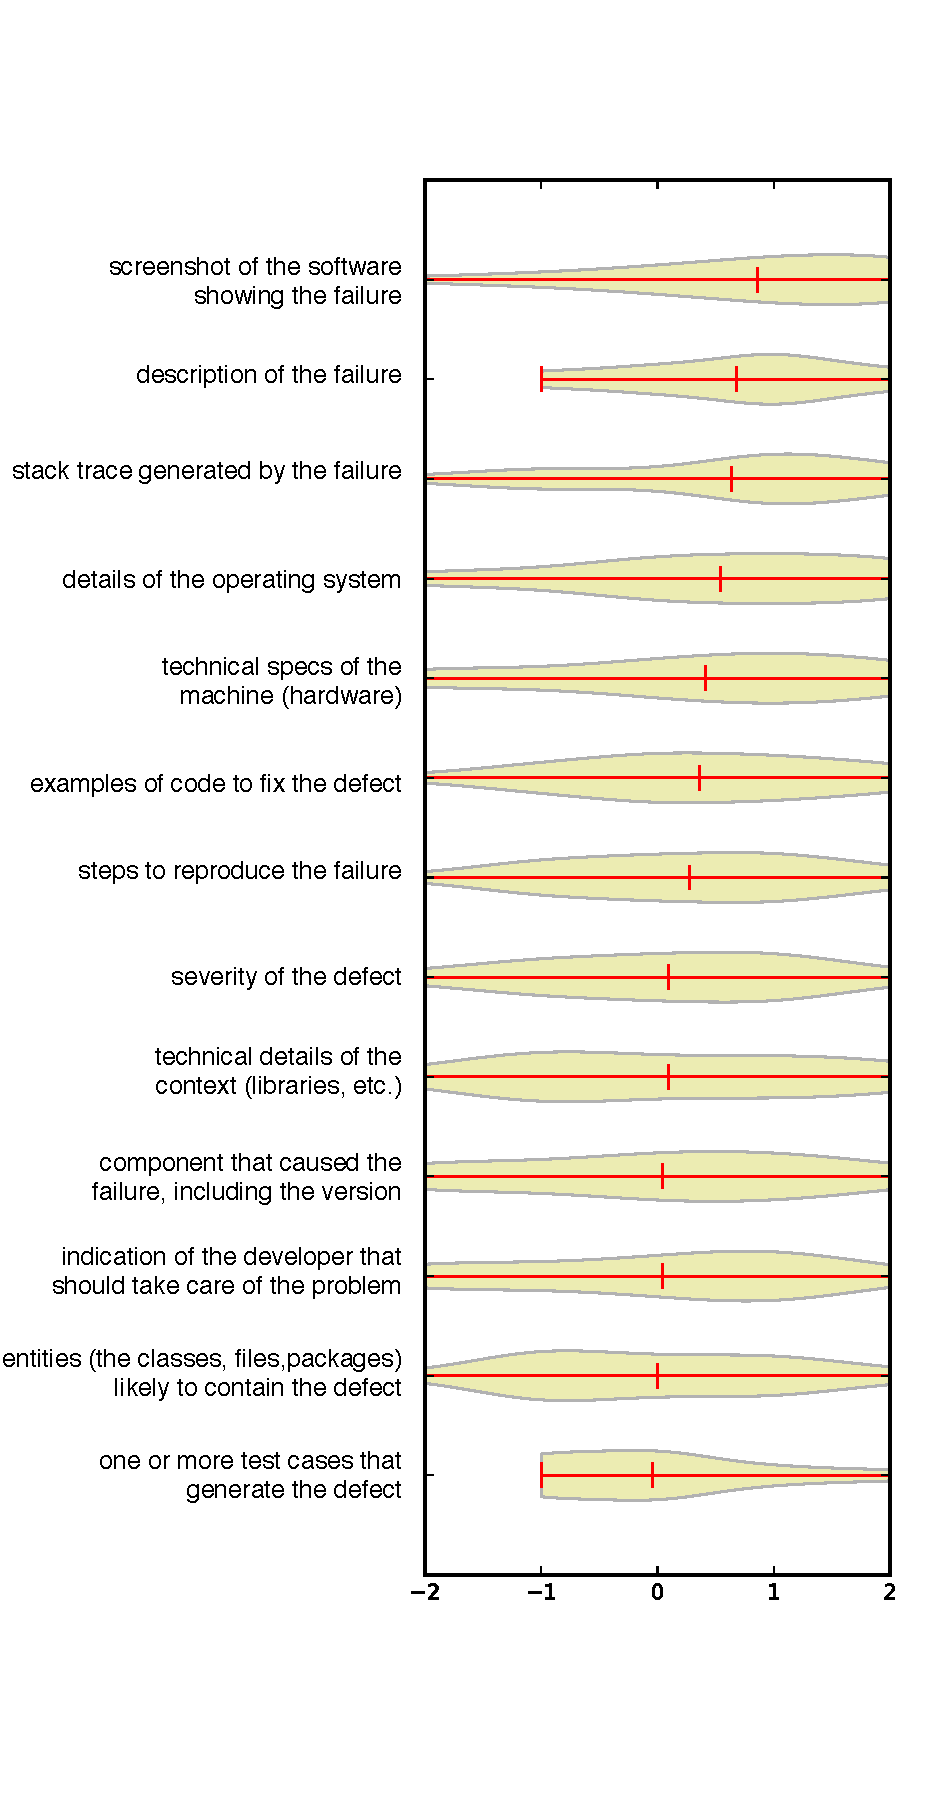
\includegraphics[width=.6\linewidth]{model/survey_plot}
\caption[Survey results]{Survey results: The higher the values, the easier it is to provide the corresponding information, according to the respondents' perception.}
\label{fig:survey}
\end{figure}
%
The majority of the users does not find excessively hard to provide most of the elements.
This is due to the fact that the Pharo community is composed of experienced programmers.
Interestingly, finding the assignee is not considered excessively difficult: Again, this can relate to the community experience, that has a strong core of well-known developers that work as hub when dealing with defects.
The elements considered to be harder to provide are the entity (\eg class, file) that likely contains the defect, the steps to reproduce the failure, and a test case showing the defect.


\subsubsection{Conclusion}

\figref{fig:survey} shows that some elements are perceived as more difficult to provide when submitting a bug report.
There is a set of easier elements, like screenshots, descriptions of the failure, stack traces, and the details of the operating system and hardware.
Those elements are useful in identifying the defect, but are less effective than other elements we identified to support its resolution.


%%%%%%%%%%%%%%%%%%%%%%%%%%%%%%%%%%%%%%%%%%%%%%%%%%%%%%%%%%%%%%%%%%%%%%%%%%%%%%%%%%%%%%
\begin{figure*}[ht]
\centering
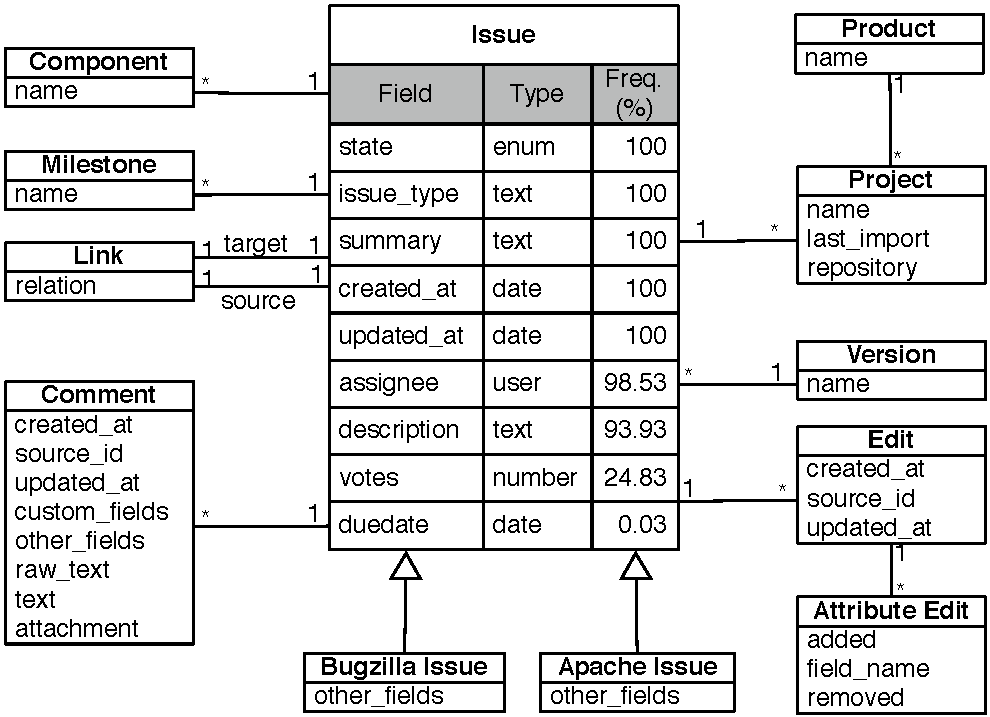
\includegraphics[width=.9\linewidth]{model/model}
\caption{Conceptual diagram of the model of a new bug report}
\label{fig:model}
\end{figure*}

\subsection*{RQ2: What is a comprehensive unified meta-model for describing data from different bug tracking systems?}\label{sec:model-model}

To devise a unified meta-model for the data we collected from the different issue trackers, we extract the model for each separate platform by reverse engineering the data and by using the documentation for the various trackers.
We identify the entities that compose a bug report, the fields  composing it, and the relation between the various entities.
We intersect the list of each bug report and select the most common ones, to summarize the salient traits of a bug report.


\subsubsection{Anatomy of a Report}
Issue trackers are platform independent: They share a flexible common core structure to meet all the possible requirements of a software system's development process.
A bug report is then built around a text description of an issue, where the user can specify the steps to reproduce the issue or include snippets of code that exemplify the context where the issue may happen.

The text description is complemented by additional metadata, used to improve the report and to track the evolution of the bug, and it can also contain attachments, like stack traces and patches.
While the description of the issue and the possibility to attach files is common to all issue trackers, the metadata used to integrate the description differ in each platform.
We can classify these attributes in three layers:

\begin{itemize}[$\circ$]
 \item \textit{Common:} metadata in every report in each platform, \ie the core set of attributes that describes a bug report.
 \item \textit{Platform specific:} metadata that are used throughout a single platform.
 \item \textit{Project specific:} custom metadata set by the users, used in a single project.
\end{itemize}


\subsubsection{The Model}

From the list of entities in a tracker and their list of metadata, we built a model to access the data.
Given our focus, we present a view of the model from the submitter's point of view.
\figref{fig:model} shows the conceptual diagram of the unified model for a typical bug tracking system with the frequencies of use for the common fields and trimmed of the post-report information.
%The diagram is composed of the following entities:


\begin{itemize}[$\circ$]
\item \textit{Issue:} The main entity representing a bug report, with the text description and the metadata provided by the user.
\item \textit{Comment:} User-provided additional information on a report.
\item \textit{Edit:} A change in the existing report.
It can group several changes.
\item \textit{AttributeEdit:} A change to a single element: It contains the modified attribute, the added, and removed text.
\item \textit{Link:} The relation (if any) to another report.
A link maps the connection and defines the type of relation (\eg parent or duplicate).
\item \textit{Project:} The project the issue tracker refers to (\eg Firefox).
\item \textit{Product:} A single instance of an issue tracking platform (\eg Bugzilla or JIRA).
\item \textit{Component:} The area of the code affected by the defect.
\item \textit{Versions:} The software version(s) where the bug was observed.
\item \textit{Milestone:} The software version(s) targeted for a fix, for planning purposes.
\end{itemize}

There are additional attributes that are not present in every platform.
To map these specific elements, there are entities that derive from \textsc{Issue} (\eg \textsc{Bugzilla\_Issue}).

These entities contain the fields \texttt{other\_fields} and \texttt{custom\_fields}.
These are two \emph{dictionary} fields that collect all the fields that are not represented in each model, in an unstructured fashion.
The field \texttt{other\_fields} contains the information from a specific bug tracker, shared in all the projects in that database (like the field \texttt{alias} in \bzilla).
The field \texttt{custom\_fields} contains non standard attributes that are customized by the maintainer of each project.
For example, the attribute \texttt{cf\_status\_firefox41}, of the project \textsc{Firefox} in \bzilla.
Some fields may seem redundant: For example, the field \texttt{updated\_at} of \textsc{Issue} could be derived by the information contained it the \textsc{Edit}s; we tolerate a small degree of duplication of the data, in exchange for flexibility and completeness with different bug reporting systems.



%%%%%%%%%%%%%%%%%%%%%%%%%%%%%%%%%%%%%%%%%%%%%%%%%%%%%%%%%%%%%%%%%%%%%%%%%%%%%%%%%%%%%%

\subsection*{RQ3: What are the recurrent states and transitions in reports?} \label{sec:model-approach-states}

We tracked the evolution of bug reports using the \texttt{state} attribute, which is an enumeration from a set of predefined states.
\tabref{tab:dataset-statuses} shows the states used in the two bug trackers we consider.
Each platform proposes different conventions to map the state of a report.
Often, different projects use the same states in a different context and a different distribution, \eg bug reports in \jira converge toward the \textsc{Closed} state, while in \bzilla they converge toward a state called \textsc{RESOLVED}.
We analyze the state changes by building a transition graph, with an approach similar to the one used by D'Ambros \etal~\cite{DAmb2007b}.

\figref{fig:apache_transitions} and \figref{fig:mozilla_transitions} show the transition diagrams for \jira and \bzilla obtained by the collected data.

\begin{figure*}[t]
\centering
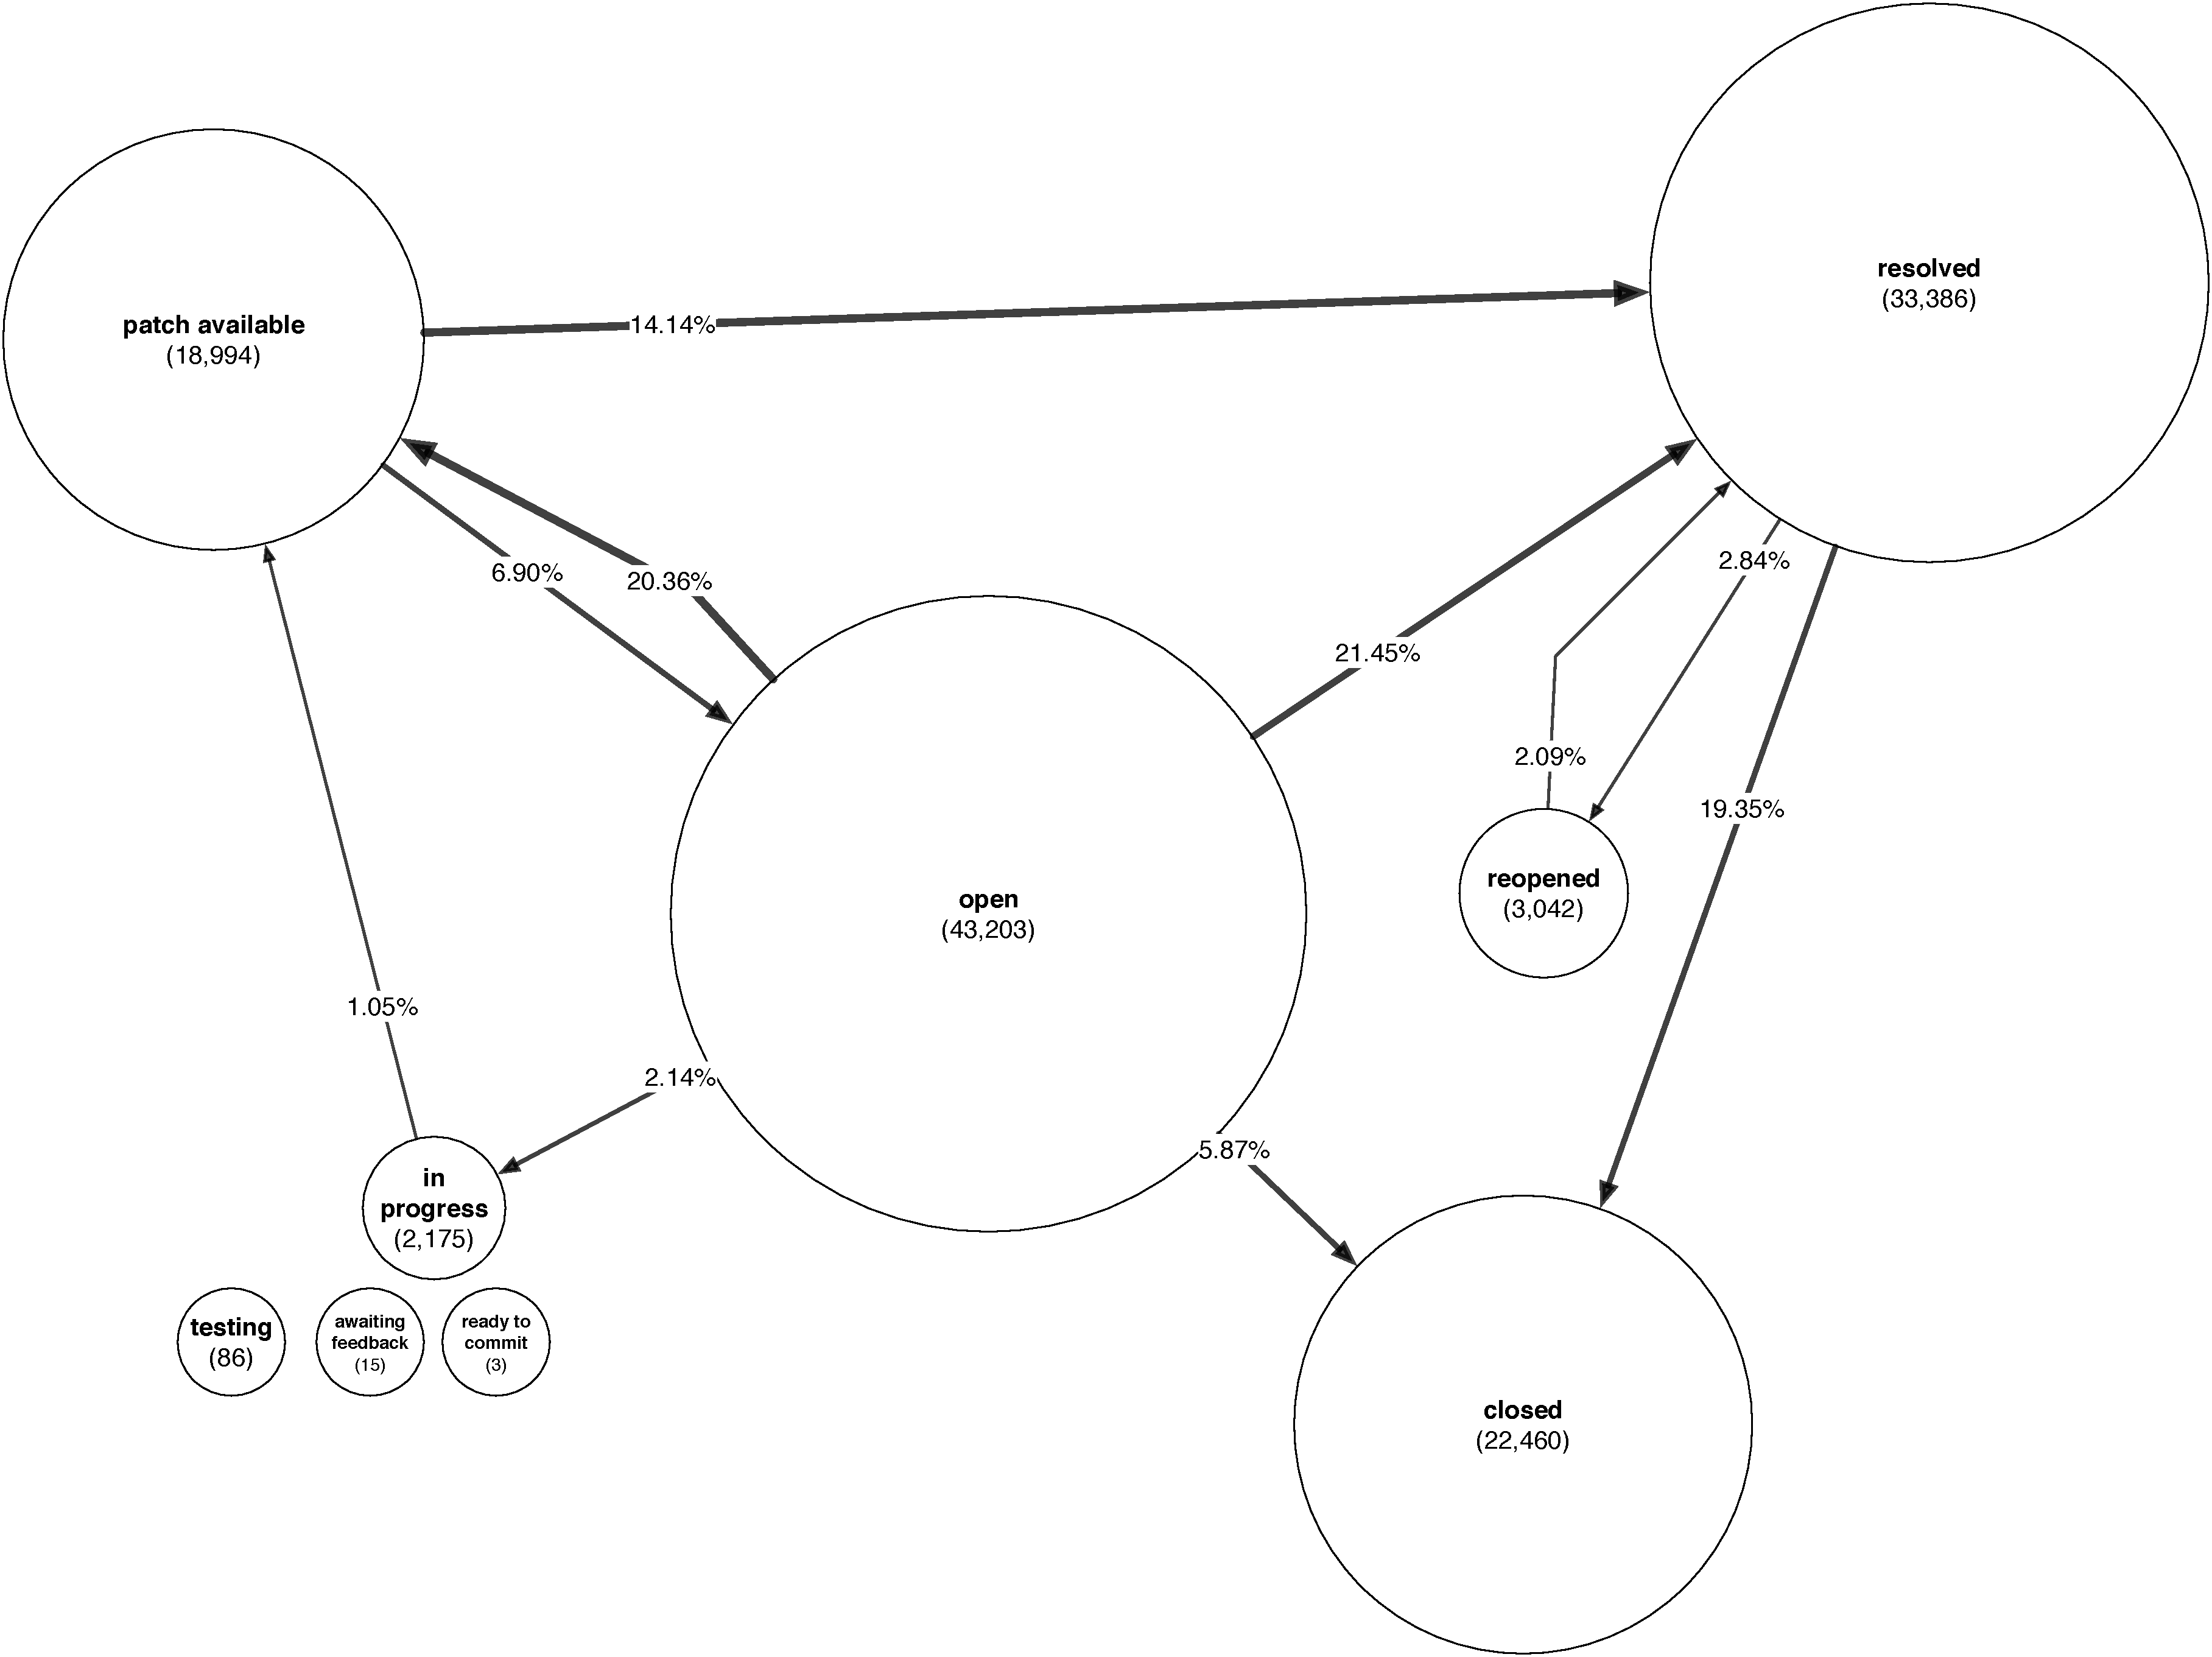
\includegraphics[width=.99\linewidth]{model/apache-transition-diagram}
\caption{Transition graph of all the states in \jira}
\label{fig:apache_transitions}
\end{figure*}

In the diagrams each node is a state, where the area grows with the number of reports that traverse that state, as presented in \tabref{tab:dataset-statuses}.
Each arc between two states indicates a transition from one state to another and its width represents the total number of transitions.
The diagram excludes all edges that make up less than $1\%$ of all the transitions.
Given \figref{fig:apache_transitions} and \figref{fig:mozilla_transitions} we can classify the states in three groups:

\begin{itemize}[$\circ$]

\item \textit{Active states:} The first group contains the most active states (\ie touched by the majority of bug reports), that are often involved in loops between them.

\item \textit{Intermediate states:} These states (\eg \textsc{testing}, \textsc{in progress}, \textsc{reopened}) indicate states where an action is taking place or expected (\eg a patch is waiting for review or the continuous integration server is running the tests).

\item \textit{Unused states:} Some states are rarely used: \textsc{awaiting feedback} and \textsc{ready to commit}.
They represent some corner cases that detail extremely specific aspects of the fixing activity.
Their very low usage may hint at a little interest in tracking these aspects in this way.

\end{itemize}

The analysis highlights that some projects do adopt customized states to track the intermediate aspects of their projects' workflow, but they tend to be not used in practice.

\textbf{Conclusion.} The analysis on the usage of the states in \secref{sec:model-approach-states} seems to suggest that:
\begin{itemize}[$\circ$]
\item A simple model with a few states, as the one described by D'Ambros \etal~\cite{DAmb2007b}, satisfies the need of tracking the state of an issue;
\item Adding customized values to  describe additional specific and intermediate steps in the fixing process is not working to track a better evolution of the state of a report.
\end{itemize}

The latter aspect is strengthened by the fact that \jira offers less states than \bzilla, but these additional states are rarely used in practice.



%\begin{table*}[h!]
%\centering
%\caption{Number of custom fields per project}
%\begin{tabular}{|l|lrrr|}
%\hline
% & \textbf{Project} & \textbf{\# fields} & \textbf{Avg. lifetime (d)} & \textbf{Max lifetime (d)} \\
% \hline \hline
%\bzilla & Air Mozilla & 5 & 154 & 1,004 \\
% & Bugzilla & 5 & 343 & 5,650 \\
% & Core & 142 & 227 & 5,936 \\
% & Firefox & 112 & 235 & 5,314 \\
% & Firefox for Android & 89 & 76 & 2,176 \\
% & SeaMonkey & 90 & 278 & 5,437 \\
% & Thunderbird & 74 & 259 & 5,451 \\
%\hline \hline
%\jira & Cassandra & 11 & 61 & 1,728 \\
% & Hadoop & 13 & 172 & 3,012 \\
% & Lucene & 13 & 182 & 3,787 \\
% & Mahout & 11 & 94 & 1,235 \\
% & Maven & 9 & 402 & 3,443 \\
% & Pig & 11 & 72 & 2,149 \\
% & Sorl & 7 & 148 & 2,858 \\
% & Zookeeper & 12 & 158 & 2,108 \\
%\hline
%
%
%\end{tabular}
%\label{tab:project-fields}
%\end{table*}

%%%%%%%%%%%%%%%%%%%%%%%%%%%%%%%%%%%%%%%%%%%%
\subsection*{RQ4: Does the completeness of standard and project-specific attributes in a bug report relate to its lifetime?}\label{sec:model-fields}

% \AB{It seems strange to me that this section ends here.
% Is the following the actual results on 'custom fields having a measurable impact on the resolution'? It should be in my opinion, so I would recommend having one single section.
% But after reading the next section it is much more than that.
% I think this part and the next subsection should be restructured.
% For example, start from the large lifetime of a report and then investigating the effect of the customized fields.
% This means moving the subsection above near the end of the next one, but not as a separate subsection.}

To investigate the impact that the fields have on solving a defect, we considered the \emph{lifetime} (defined as the time to the final fix) of the closed reports.

In addition to its standard set of attributes, each issue tracker we consider allows projects to define additional fields to customize the structure of a bug report.
In our study, we group all the attributes in three \emph{layers}:

\begin{itemize}[$\circ$]
\item \textit{Core Fields:} The fields that are common to all projects and all the issue trackers.
They map the essential information to describe a software defect;
\item \textit{Tracker-Specific Fields:} The fields that are shared among all the projects in an issue tracker, but are not present in all the platforms;
\item \textit{Project-Specific Fields:} The fields that are customized by the user and appear only in a single project.
\end{itemize}

Each project in our dataset specifies its own set of custom fields.
We also investigate whether these fields have a measurable impact on the lifetime of a bug report.

\begin{figure}[t]
\centering
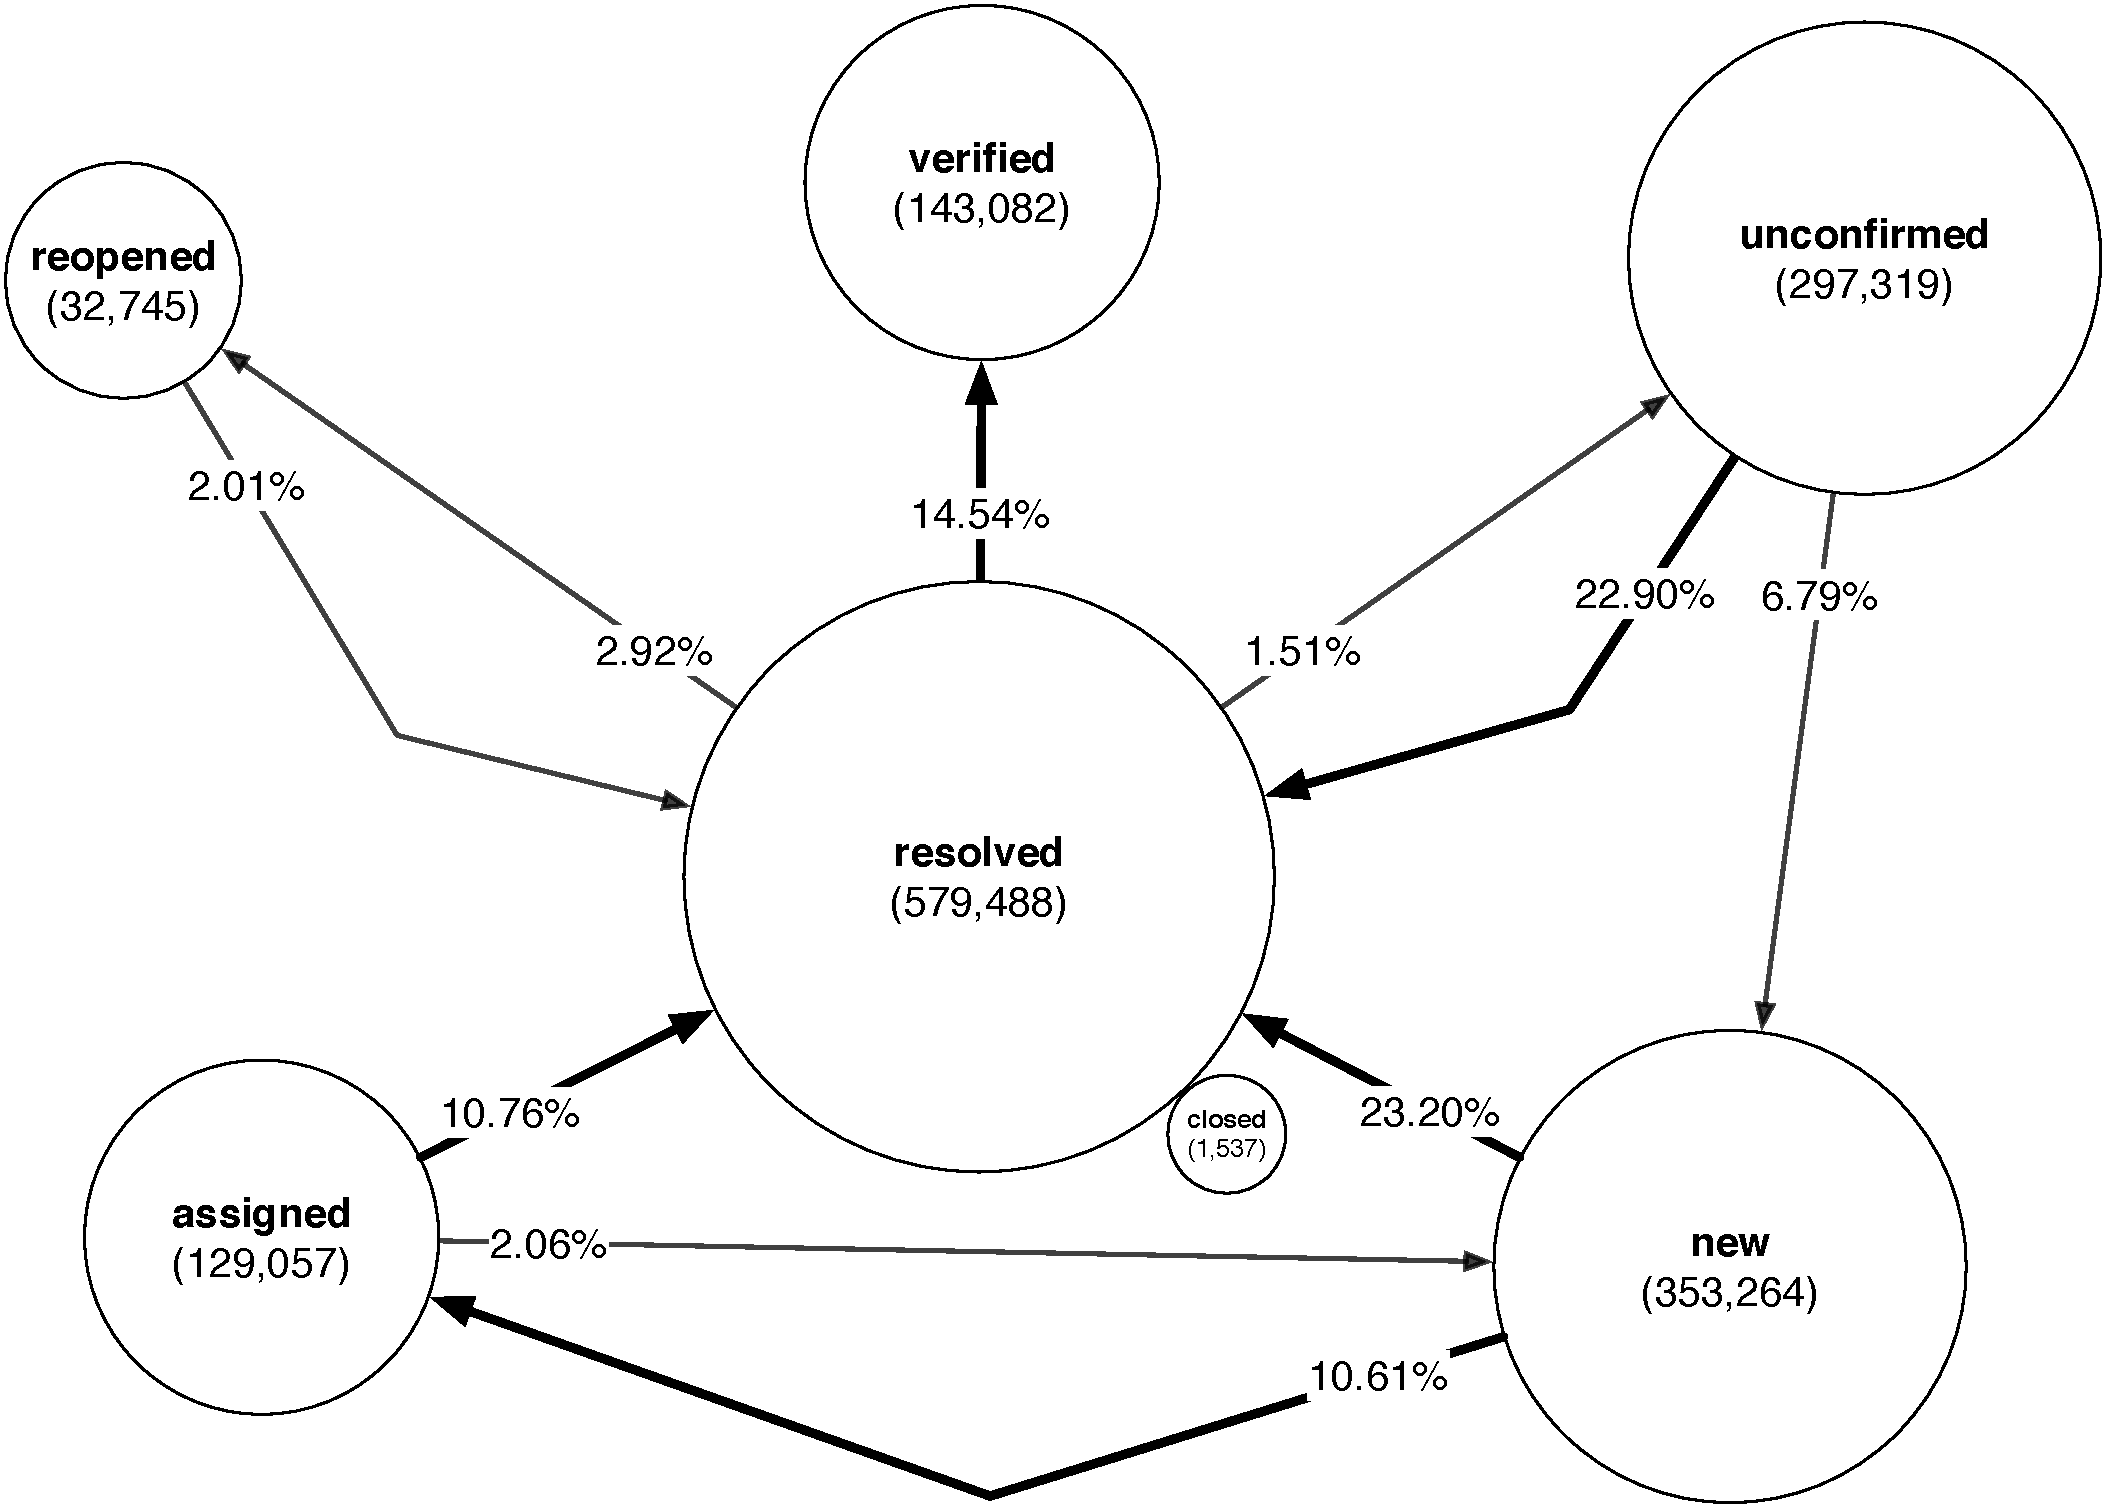
\includegraphics[width=.9\linewidth]{model/mozilla-transition-diagram}
\caption{Transition diagram of all the states in \bzilla}
\label{fig:mozilla_transitions}
\end{figure}

 \tabref{tab:project-fields} shows a count of project-specific attributes in our dataset, including the average and maximum lifetimes of the corresponding bug reports, reported in days.

\begin{table}[ht]\small
\centering
\caption{Number of custom fields per project}
\rowcolors{1}{tablefirstrow}{tablesecondrow}
\begin{tabular}{l|rrr}
\rowcolor{tableheader}\textbf{Project} & \textbf{\# of fields} & \textbf{Avg.
lifetime (d)} & \textbf{Max lifetime (d)} \\
 \hline
Air Mozilla & 5 & 154 & 1,004 \\
Bugzilla & 5 & 343 & 5,650 \\
Core & 142 & 227 & 5,936 \\
Firefox & 112 & 235 & 5,314 \\
Firefox for Android & 89 & 76 & 2,176 \\
SeaMonkey & 90 & 278 & 5,437 \\
Thunderbird & 74 & 259 & 5,451 \\
\hline
Cassandra & 11 & 61 & 1,728 \\
Hadoop & 13 & 172 & 3,012 \\
Lucene & 13 & 182 & 3,787 \\
Mahout & 11 & 94 & 1,235 \\
Maven & 9 & 402 & 3,443 \\
Pig & 11 & 72 & 2,149 \\
Sorl & 7 & 148 & 2,858 \\
Zookeeper & 12 & 158 & 2,108 \\
\hline
\end{tabular}
\label{tab:project-fields}
\end{table}


We now explore the relationship between the various attributes adopted by the different platforms and projects we considered and the effectiveness of a bug report, measured as its lifetime.


\subsubsection{Preparing the data} To interact with the dataset, we created a \emph{vector space model} to allow us to test statistical and machine learning approaches.
Predicting the exact lifetime of a report would be unpractical and unnecessary: a timeframe for the resolution would provide a useful, human-understandable measure, while allowing more accurate predictions.
To introduce such a degree of tolerance, we divide the reports into \emph{buckets} according to their lifetime.

 Using bucketing we can deal with discrete values and adopt a classification approach, as opposed to a regression to predict a continuos variable.
We split the lifetime space into four buckets: less than one day, less than one week, less than one month, and more than one month.
We chose these intervals because they reflect humane time periods and they describe increasing timespans, reflecting that the longer a bug report stays open, the less relevant its exact resolution time becomes.
After bucketing the issues, we model each report as a vector of booleans (each field maps an attribute of the report and its value is 1 iff the user filled it) and associate it with its classification into a bucket of lifetime, which we can feed to different prediction algorithms.


%%%%%%%%%%%%%%%%%%%%%%%%%%%%%%%%%%%%%%%%%
\subsubsection{Principal Component Analysis}\label{sec:model-pca}

To understand the relation between the completeness of a bug report and the fixing time of a defect, we want to inspect how much each field contributes to  the lifetime of a bug report.

For this purpose, we use \emph{Principal Component Analysis} (PCA)~\cite{Abdi2010a} to extract the variance between the different fields.
PCA is a statistical procedure that aims to extract only the salient features from a data table.
PCA transforms the existing data into variables called \emph{principal components}, which are described as a linear combination of the existing features.
The other features are then projected on the principal components.


The components extracted by PCA represent the eigenvectors of the covariance matrix.
Internally, PCA implements a \emph{single value decomposition} to extract the scores of the factors.
%PCA calculates the correlation between the components and projects the instances of the dataset using the components.
The number of components to extract is an open problem, but generally, when solving a correlation problem, PCA keeps the components that have an eigenvalue above the average.

We use PCA to determine which combination of fields carries the most information with respect to the lifetime of a defect, by observing which elements are selected to compose the principal components.
To interpret the results and obtain a general set of fields that influence the lifetime of a bug report, we consider the core fields of the projects.
This operation gives us the important fields that impact the lifetime of a bug report.

After running PCA, we obtain a set of new components that can be used to map the dataset.
We are not interested in the new features per-se, but --- since the features of the dataset are the fields of the bug reports --- we investigate which original features were selected to describe the components.

We then inspect how the components are calculated, obtaining the following selected fields:

\begin{itemize}[$\circ$]
  \item \emph{assignee\_id}: the person the bug report is assigned to;
  \item \emph{creator\_id}: the person that submitted the bug report;
  \item \emph{description}: the number of words in the description of a bug report;
  \item \emph{duedate}: if the bug report has a due date;
  \item \emph{reporter\_id}: the person that initially reported the defect (can be different than the creator)
  \item \emph{summary}: the number of words in the summary of the bug report.
\end{itemize}

These fields were extracted by the algorithm as the most relevant in impacting the lifetime of a bug report.
Although they do not represent the whole amount of information that is needed to describe a software defect, the fact that they were selected by PCA indicates that their contribution in determining the lifetime of a report is significant.
It follows that users and developers should take these elements into account when submitting a bug report and the issue tracker should ensure that these fields are exploited accordingly.

%%%%%%%%%%%%%%%%%%%%%%%%%%%%%%%%%%%%%%%%%%%%%%%%
\subsubsection{Predicting the Lifetime of a Defect} We studied the core fields that are the most relevant in impacting the lifetime.
Now we investigate how the lifetime gets influenced by the different fields defined by each project.
For such an analysis PCA is not suited, as the data is too sparse and the features would be discarded in the process.
We therefore adopt a \emph{machine learning} approach to estimate an approximate lifetime of a bug report given its ``completeness,'' \ie the number of completed fields when submitted.

We verify the impact on the prediction of the different levels of attributes using various machine learning algorithms on our model, by employing the \textsc{scikit-learn} analysis tools~\cite{Pedr2012}.
In particular, we used \emph{Na\"ive Bayes}~\cite{mitc1997}, \emph{Decision Trees}~\cite{mitc1997}, \emph{AdaBoost}~\cite{bish2006}, and \emph{Random Forest}~\cite{brei01} and validated our approach using $k$-fold cross-validation.
We balance the training dataset to get homogeneous buckets containing 50,000 bug reports each, to prevent the different distribution of the sets to give a bias towards the biggest buckets~\cite{bati2004}.
In this context, a random classifier would correctly classify 0.25 of the instances, so a classifier is better than random if it achieves a higher proportion.

\tabref{tab:ml-results} shows the prediction results: Each column represent a classifier, while each row represents each layer of attributes we add to the model.

\begin{table}[ht]\small
\centering
\caption{Prediction results: Proportion of bug reports classified in the correct time bucket, with increment over  random classification (25\% correctly classified bug reports).}
\rowcolors{1}{tablefirstrow}{tablesecondrow}
\begin{tabular}{l|r|r|r|r}
\rowcolor{tableheader} & \textbf{NB} & \textbf{DT} & \textbf{AdaBoost} & \textbf{RF} \\
 \hline
Common & 0.27 (+0.02) & 0.27 (+0.02) & 0.27 (+0.02) & 0.27 (+0.02) \\
+ words & 0.28 (+0.03) & 0.28 (+0.03) & 0.29 (+0.04) & 0.28 (+0.03) \\
+ tracker & 0.36 (+0.11) & 0.36 (+0.11) & 0.42 (+0.17) & 0.36 (+0.11) \\
+ project & 0.37 (+0.12) & 0.36 (+0.11) & 0.42 (+0.17) & 0.37 (+0.12) \\
\hline
\end{tabular}
\label{tab:ml-results}
\end{table}

In the first round we use the \emph{common} attributes displayed in \figref{fig:model}; in the second, we add the number of words that compose the summary and the description of the report; in the third, we add the \emph{tracker} features, \ie the attributes that appear in some issue trackers; in the last, we add the \emph{project} features, \ie the non standard attributes that are customized by the users of the platform.
We follow this order to increasingly add the more and more specific fields and evaluate the impact that the different customizations have on the overall model.
%\AB{why this order? What if I add the last layer first? It would be great to see the real statistical significance (p value?) of each set of attributes, to know which ones really matters.}
We can see from \tabref{tab:ml-results} that the best results are achieved by AdaBoost~\cite{bish2006} using the tracker-specific fields, with an overall accuracy of $0.42$.
Differently from the shared and tracker-specific fields, the project-fields may vary over time.
They are, in fact, constantly added: Firefox, for example, adds a new custom field specific for each release, which happens once every 6 weeks.
This mutability can raise the question whether the contribution of these fields is diluted in such a long timespan.
To mitigate this effect, we recompute our experiments on the subset of bug reports collected in the timeframe that starts exactly one year before the dataset collection.
The new dataset is composed of 31,472 bug reports.
\tabref{tab:ml-results-fresh} shows the results of our second batch of experiments.

\begin{table}[ht]\small
\centering
\caption{Prediction results for bug reports of last year.}
\rowcolors{1}{tablefirstrow}{tablesecondrow}
\begin{tabular}{l|r|r|r|r}
\rowcolor{tableheader} & \textbf{NB} & \textbf{DT} & \textbf{AdaBoost} & \textbf{RF} \\
 \hline
Common & 0.27 (+0.02) & 0.28 (+0.03) & 0.28 (+0.03) & 0.28 (+0.03) \\
+ words & 0.30 (+0.05) & 0.30 (+0.05) & 0.33 (+0.08) & 0.30 (+0.05) \\
+ tracker & 0.34 (+0.09) & 0.37 (+0.12) & 0.46 (+0.21) & 0.39 (+0.14) \\
+ project & 0.35 (+0.10) & 0.39 (+0.14) & 0.46 (+0.21) & 0.42 (+0.17) \\
\hline

\end{tabular}
\label{tab:ml-results-fresh}
\end{table}

Indeed, the results on the most recent dataset do not differ significantly from the results based on much longer timespans.

\textbf{Conclusion.} From our study using PCA, we observe that there exists a set of core elements of a bug report that impact and influence its lifetime.
Comparing these result with the perceived difficulty presented in RQ1, we see that some of these elements, like a description of the problem, the screenshot or the stack trace, compose the description field that we saw impacting the resolution time.
Another relevant element is the assignee of the report, but users find it hard to provide it.
Interestingly, the elements that are the most useful in the resolution of a software defect are also harder to provide.
From the experience with the various issue trackers and their interfaces, we believe that a user submitting a bug report should be offered a clean interface, that minimizes the amount of required information, highlights the most effective elements, and progressively requires the harder or less relevant ones.
The AdaBoost machine learning model achieves the best results, yet it can only predict the lifetime of a limited number of bug reports.
The increment over a random classifier prediction is particularly small for the \emph{common} attributes.
This can be explained by the terse nature of the core model.
Moreover, the \emph{tracker} fields improve prediction, showing a relation between more detailed bug reports and bug lifetime.

After calculating the lifetime of each bug report in the tracker, we compare data from the two considered platforms.
By analyzing the average lifetime of the bug reports in each platform we note that they have a longer lifespan on \bzilla than on \jira, with an average fixing time of 239 and 166 days, respectively.
Even if the longer life of \bzilla projects may explain this phenomenon, we measure a gap between the lifetime of the reports in the two platforms (109 days for \bzilla and 93 days for \jira), even when we restrict ourselves to consider reports submitted after 2009 (\ie when all the projects were active).
There is an interesting, unexplained substantial difference in the way bug reports are processed in the two platforms.
Studies can be designed and carried out to determine whether and how the bug reporting system itself leads to this behavior or there is a possibly unconscious self-selection of projects in using one or the other system.
Concerning project-specific attributes, from the results of the test, depicted in \tabref{tab:ml-results} and \tabref{tab:ml-results-fresh}, it emerges that they have the least weight in predicting the lifetime of a report.
This suggests that they are not related to the fixing time.
This may be a hint that these fields probably track collateral aspects of the evolution of a report that are not related to how quick a bug will be solved.

Last, we examine which fields impact the prediction the most: They are the number of words of the description and the summary, suggesting that an accurate description of the problem is important to engage the developers.
The fields that connect the issue with other reports are also relevant, for example the dependent issues, as well as the fact that a bug report is already assigned at the time of submission.



\section{Discussion}\label{sec:model-discussion}

This section discusses the possible problems of our approach and how our work can be improved.


\subsection{Threats to Validity}

Dealing with large amounts of data can pose some problems in creating an abstraction sufficiently broad to comprise all the aspects of the data, but still specific enough to capture its details.
We spent a considerable amount of time dealing with the representation of the data, extracting its features and cleaning the unneeded parts.
In particular, we carefully excluded from our prediction model all the fields that could yield a-posteriori information on the lifetime of a report.
In a large dataset it is hard, however, to guarantee the complete soundness of the whole corpus, that could contain hidden relations between some attributes.

There is the concern that the lifetime of a bug report, that we used as a measure of quality of a bug report, is not relevant for our task.
However, this metric proved to be an interesting open problem in the field and it represents an interesting heuristic in determining the effectiveness of a report.


\subsection{Next Steps}

Developers tend to prefer simpler models to depict software defects.
Even when provided with customization means, the additional information did not show a correlation with the lifetime of a report.
Modern issue trackers like \jira and \bzilla are complex interfaces over a set of tables in a relational database and the need for additional features over time makes those platforms grow over time, progressively turning them into inflexible \emph{colossi}.

GitHub adopts the opposite approach, by providing a minimal structure of a bug report that is mostly a note attached to a commit or a piece of code.
This interesting approach, however, lacks the descriptive power of the other two platforms.
The need for a simpler model is hinted by the choices of the development team of \bzilla that on version 5.0, released in July 2015, proposes a simplified interface that asks the user for a summary and a description of the problem, polished of all the additional information.

We believe that the future of issue tracking systems lies in flexible structures that can dynamically adapt to different aspects of the development activity.


% %%%%%%%%%%%%%%%%%%%%%%
% \section{Related Work} \label{sec:model-related}
% %%%%%%%%%%%%%%%%%%%%%%
%
% Dealing with bug reports is a non-trivial task: Not only do users have to report meaningful information and developers have to understand and reproduce a problem, but they also have to deal with the large, noisy, and sometimes duplicated  information stored in issue tracking systems.
% To minimize the impact that dealing with reports has on the bug fixing activity, researchers proposed different approaches to support developers and to automate important steps.
%
% \textbf{Reliability of a Bug Report.} The first important aspect involving bug reports is the reliability and completeness of the information contained in a report.
% Through questionnaires, researchers collected information on how developers perceive the quality of a bug report and consider the most influential elements that help understanding a problem~\cite{Zimm2010a,Bett2007,Schr2010a}.
% Researchers also proposed techniques to detect and avoid bug reports that do not contain useful information~\cite{Sun2011}, thus alleviating the developers from information overload.
% Bissyand\'e \etal investigated the impact of the issue tracker on the development of a project~\cite{Biss2013b}, finding that most bug reporters are not developers of the project.
%
% \textbf{Automating Management of Bug Reports.} Researchers proposed different approaches to automate bug report processing~\cite{Weim2006}.
% For example, a crucial aspect of managing bug reports is finding the ideal person to take care of an issue, known as {\em triaging}; Anvik \etal proposed a machine learning based approach to automate this step~\cite{Anvi2006a}.
% Guo \etal conducted a study to predict the aspects that impact the resolution time of \textit{MS Windows} bug reports~\cite{Guo2010}.
% They found that a high number of reassignment of a report decreases the likelihood of the report of being closed quickly.
% They also found that the reputation of the submitter is an important factor to shorten the fixing time.
% Given the expensive nature of the bug fixing activity, Weiss \etal devised an approach to estimate the cost of a bug fix in person-hours~\cite{Weis2007a}.
% Giger \etal studied the issue tracker of different open source project to predict bug fixing time, finding that the assignee and the reporting month are strong predictors~\cite{Gige2010}.
% Also, post-release information like the assignee is useful in increasing the accuracy.
% Bhattacharya and Neamtiu showed the low correlation of current prediction techniques and underlined the need to find additional attributes to increase the confidence of the time estimates~\cite{Bhat2011}.
%
% \textbf{Bug Reports and Social Interactions.} An issue tracker represents also a social aspect of the community: users can interact with developers and provide feedback in fixing a defect.
% Breu \etal performed an analysis on a sample of 600 bug reports, finding that interacting with developers provides help in fixing the defect~\cite{Breu2010}.
% Zhou and Mockus showed that users involved in the development activity, like bug reporting and participating in the community, are more likely to become stable, long time contributors~\cite{Zhou2015}.
%
% \textbf{Bug Report Databases Visualization.} Researchers proposed a number of visualizations to analyze feature of the bug reporting systems.
% For example, D'Ambros \etal performed an analysis of the \bzilla bug repository: They summarized the diagram of the state transitions of a report and proposed a set of visualizations to support the analysis of a bug database at different levels of granularity.
% Their approach allows the user to navigate the history of a single issue tracker and inspect selected part of the system with customized filters~\cite{DAmb2007b}.



%%%%%%%%%%%%%%%%%%%%
\section{Outline} \label{sec:model-summary}
%%%%%%%%%%%%%%%%%%%%

We conducted an investigation to identify the features that are relevant to obtain a \emph{satisficing} bug report.
In doing so, we provided the following contributions:

\begin{enumerate}
\item An overview of the perceived difficulty of submitting elements of a bug report for users;

\item A meta-model for bug reports that represents both the common and specific elements available in reports of different issue trackers;

\item A publicly available dataset of more than 650,000 bug reports, modeled according to our meta-model;

\item An analysis of the contents of the issue trackers, to identify features that are related to reports' lifecycle;

\item Evidence that increasing the number of fields provided when submitting a bug report has little relation on shortening the lifetime of a bug.

\end{enumerate}


This chapter concludes our discussion about collecting information about bugs.
We proposed different approaches to support developers in their bug fixing activity.
We used automation to collect reliable data, we built visualizations to provide effective access to the data, and we discussed how we can improve the model of a bug report.
We are still left, however, with the issue that bug fixing is intrinsically a boring and tedious activity.
In the next chapter we try to mitigate this problem by exploring the field of \emph{gamification}, investigating whether its use can help developers and communities in processing the large amount of unstructured information that populates issue tracking systems.
